%----------------------------------------------------------------------------------------
%	PACKAGES AND OTHER DOCUMENT CONFIGURATIONS
%----------------------------------------------------------------------------------------
\documentclass[preprint, twocolumn, 5p, lefttitle]{elsarticle} %lefttitle per mettere il titolo a sinistra, altrimenti viene messo al centro. % 5p per avere il testo più esteso sul foglio (altrimenti 1p o anche 3p)
\usepackage[utf8]{inputenc}
\usepackage[T1]{fontenc}
\usepackage[utf8]{inputenc}
%!TEX encoding = UTF-8 Unicode
\usepackage{geometry}
\usepackage{geometry}% Pacchetto per modificare lunghezza e layout di alcuni elementi 
\usepackage{multicol}
\setlength{\columnsep}{0.55cm}% Distance between the two columns of text
\usepackage[numbers]{natbib}
\usepackage{amsmath}
\usepackage{capt-of}
\usepackage{dblfloatfix}% Fondamentale per mettere le figure a singola colonna anche se ne sto usando di più
\usepackage{blindtext}
\usepackage{fancyhdr}
\usepackage{lastpage}
\pagestyle{fancy} %Per aggiungere il titolo del paragrafo in alto e in maiuscolo.
\fancyhf{}
\fancyhead[LE,RO]{\fontsize{10}{12}\nouppercase\rightmark}%Per aggiungere il titolo del capitolo in alto a sinistra 
\fancyhead[RE,LO]{\fontsize{10}{12}\nouppercase\leftmark}%Per aggiungere il titolo del paragrafo in alto a destra. 
\rfoot{\thepage \hspace{1pt} / \pageref{LastPage}}
\usepackage{lipsum}
\usepackage{multicol, blindtext}
\usepackage[italian]{babel} 
\pdfpagewidth
\paperwidth
\pdfpageheight
\paperheight
\usepackage{booktabs}
 \usepackage{siunitx}
%----------------------------------------------------------------------------------------
%	HYPERLINKS
%----------------------------------------------------------------------------------------
 \usepackage{hyperref}
\hypersetup{
    colorlinks=true,
    linkcolor=blue,
    filecolor=magenta,      
    urlcolor=cyan,
}

\usepackage{graphicx}
\usepackage{color}
\usepackage{subfig}
\usepackage{verbatim}
\newcommand*{\unit}[1]{\ensuremath{\mathrm{\,#1}}}
\usepackage{amsthm}
\usepackage{epsfig}
\usepackage{booktabs} % Pacchetto per inserire tabelle 
\usepackage{longtable} % Pacchetto per tabelle molto lunghe (più di una pagina)
\usepackage[rightcaption]{sidecap}
\sidecaptionvpos{figure}{c}
\usepackage{fancyhdr} 
\usepackage{verbatim}
\usepackage{amsmath,amssymb}
\usepackage{amscd} 
\usepackage[T1]{fontenc} 
\usepackage[utf8]{inputenc} 
\usepackage[usenames,dvipsnames]{xcolor}
\usepackage{graphicx,color,listings}
\usepackage{hologo}
\frenchspacing 
\usepackage{float}
\usepackage{lettrine}
\usepackage{siunitx}
\usepackage[many]{tcolorbox}
\tcbset{highlight math style={enhanced,
  colframe=red,colback=white,arc=0pt,boxrule=1pt}}
  \tcbset{highlight math style={enhanced,
  colframe=red!60!black,colback=yellow!50!white,arc=4pt,boxrule=1pt,
  drop fuzzy shadow}}
\usepackage{rotating}
\usepackage{caption}
\usepackage{blindtext}
\captionsetup{labelformat=empty, textfont=sl}
\usepackage{placeins}
\usepackage{hyperref}
\usepackage{listings}
% TO PUT FIGURE IN MULTICOLUMNS
\newenvironment{Figure}
  {\par\medskip\noindent\minipage{\linewidth}}
  {\endminipage\par\medskip}
\usepackage{xcolor}
\definecolor{mygray}{RGB}{245,245,245}
\definecolor{ipython_bg}{RGB}{247, 247, 247}
% Per inserire codice Python.
\lstset
{ %Formatting for code in appendix
    language = Python,
    %frame       = single
    frame=single,
    %framexleftmargin=0.5em
    %framexrightmargin=0.5em
    basicstyle = \footnotesize,
    numbers   =  left,
    stepnumber = 1,
    showstringspaces = false,
    tabsize=1,
    basicstyle           = {\normalsize\ttfamily},
    keywordstyle      = \color{blue},
    commentstyle     = \color{teal},
    stringstyle           = \color{red},
    numberstyle       = \scriptsize\color{gray},
     %backgroundcolor  = \color{codebackground},
    breaklines=true,
    breakatwhitespace=false,
     backgroundcolor=\color{ipython_bg},
}
%\lstset{caption={Insert code directly in your document}}
%----------------------------------------------------------------------------------------
%	ARTICLE INFORMATION
%----------------------------------------------------------------------------------------
\frenchspacing
\title{\textbf{Titolo principale del documento \\ Sottotitolo del documento}}
\author{Lorenzo Marini \\ \texttt{lorenzo.marini.1996@gmail.com}}
%\ead{lorenzo.marini.1996@gmail.com}
%\address[mymainaddress]{Affiliation}
\begin{document}
\let\WriteBookmarks\relax
\def\floatpagepagefraction{1}
\def\textpagefraction{.001}
%\ead{lorenzo.marini.1996@gmail.com}
\begin{frontmatter}
%%%%%%%%%%%%%%%%%%%%%%%%%%%%%%%%%%%%%%%%%%%%%%%%%%%%%%%%%%%%%%%%%%%%%%%%%%%%	
\begin{abstract}
Lo scopo di questo report è quello di ... 
\end{abstract}
\begin{keyword}
Parola chiave 1\sep Parola chiave 2\sep Parola chiave 3.
\end{keyword}
\end{frontmatter}
	\newpage
	\tableofcontents
	%\listoffigures
	
%\newpage
%=====================================
% INTRODUZIONE
%=====================================
\section{Introduzione}
%\blindtext
\lettrine{Q}{uesto} documento, tratta di alcuni utili comandi da utilizzare con \LaTeX.
Ad esempio, facciamo una prova.
%=====================================
% SOTTOCAPITOLO
%=====================================
\subsection{Sottocapitolo}
\blindtext
\newline

Consultare\footnote{Esempio di nota a piè di pagina.} il repositorio \href{https://github.com/lorenzomarini96}{github}, oppure documentarsi tramite \cite{nome_da_citare} oppure, sul sito \url{https://github.com/lorenzomarini96} .
\newline

\begin{Figure}
	\centering
 	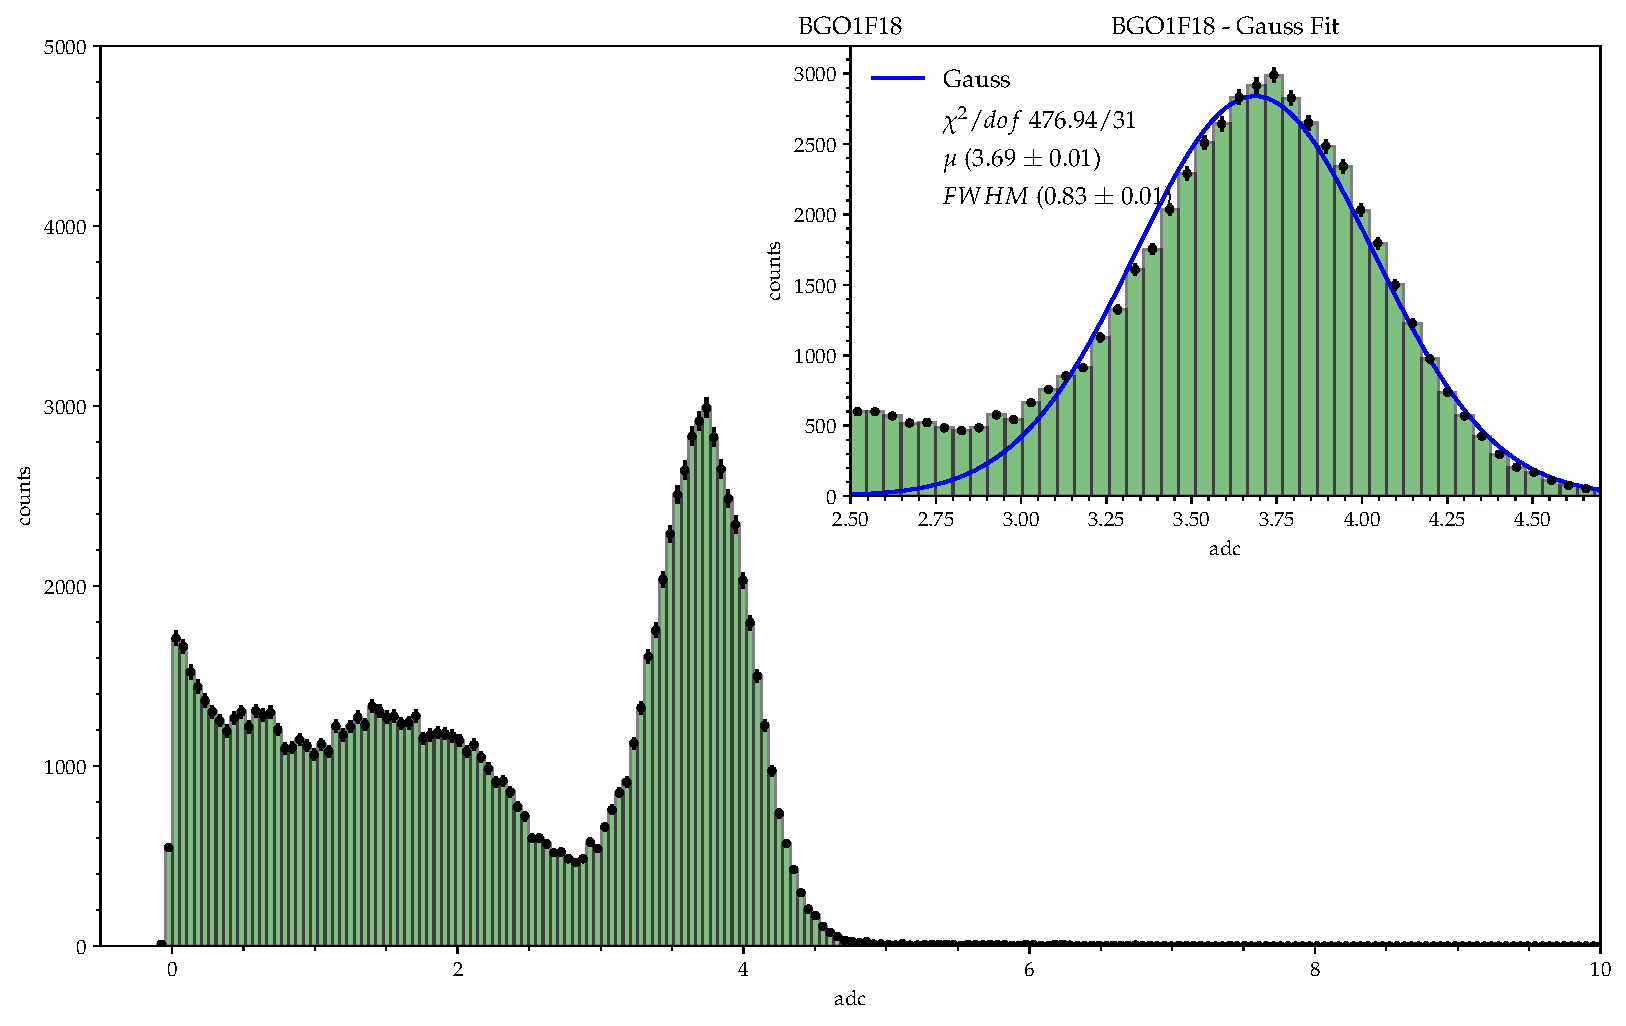
\includegraphics[width=\linewidth]{figure.pdf}
 	\captionof{figure}{my caption of the figure}
\end{Figure}

%=====================================
% SOTTOSOTTOCAPITOLO
%=====================================
\subsubsection{Sottosottocapitolo}
Importiamo un file .txt presente nella cartella di lavoro.
\verbatiminput{data.txt}

%=====================================
% EQUAZIONI IN LATEX 
%=====================================
\section{Equazioni in \LaTeX}
Esempio di equazione:

\begin{equation}
\overline{x} = \int x \> p(x) \> dx  =  \int x \> \Sigma_T \> e^{-x \> \Sigma_T} \> dx = {1\over{\Sigma_T}}
\end{equation}

\medskip

\begin{equation}
\begin{cases} \varphi &=  \varphi_{cm} \\
\cos\theta &= \frac{A\cos\> \theta_{cm} + 1}{\sqrt{A^{2} + 2A\cos\theta_{cm} + 1}}
\end{cases}
\end{equation}

\medskip

\begin{equation}
\begin{cases}
x_i = x_{i-1} + d_i\alpha\\
y_i = y_{i-1} + d_i\beta\\
z_i = z_{i-1} + d_i\gamma
\end{cases}
\end{equation}
e ovviamente $x_0 = y_0 = z_0 = 0$

\medskip

\begin{equation}
\boxed{
 x = - {1\over{\Sigma_T}} \> ln (\xi_{1})
 }
\end{equation}

\medskip

\begin{equation*}
\tcbhighmath[drop fuzzy shadow, ,watermark color=yellow!90!red]{
REID = \sum\limits_{a=a_{E}}^{a-1} m(E,a_{E},a) S(E,a_{E},a) }
\end{equation*}


%=====================================
% FIGURE IN LATEX 
%=====================================
\section{Figure in \LaTeX}
\begin{figure*}[b]
\centering
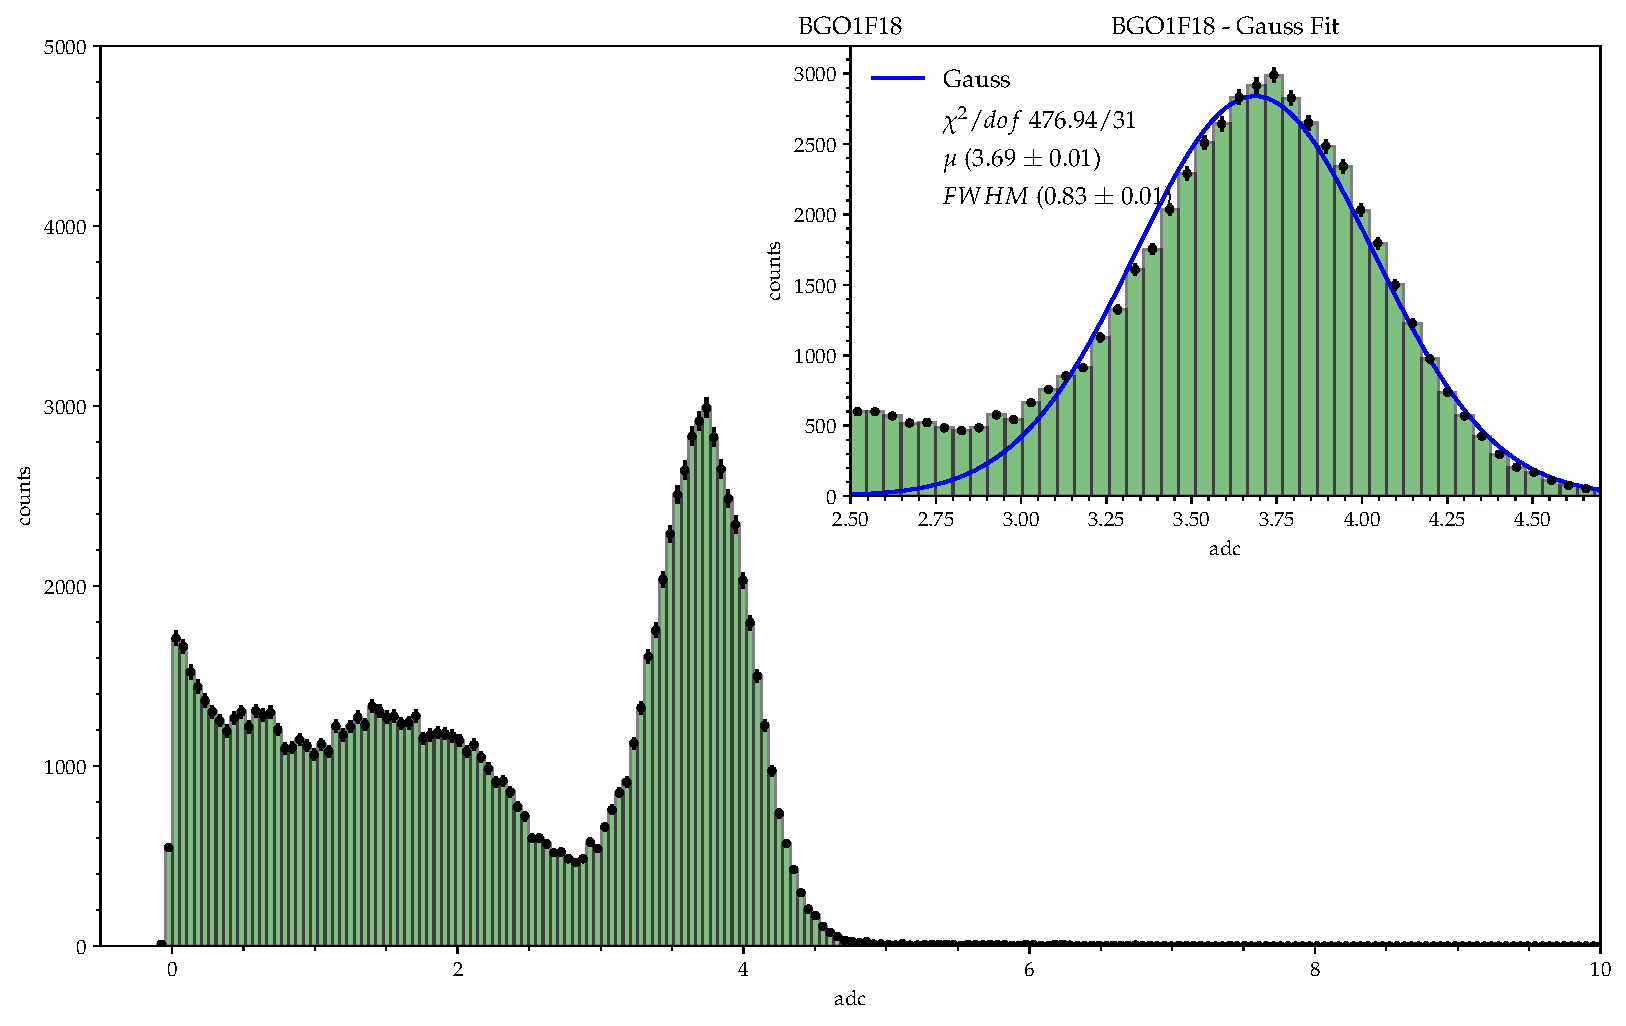
\includegraphics[width=0.80\textwidth]{figure.pdf}
\caption{Figura 1: Rappresentazione schematica della traiettoria percorsa da un neutrone $termico$ durante il suo passaggio all'interno della materia.}
\label{fig:float}
\end{figure*}
\begin{figure*}[b]
\centering
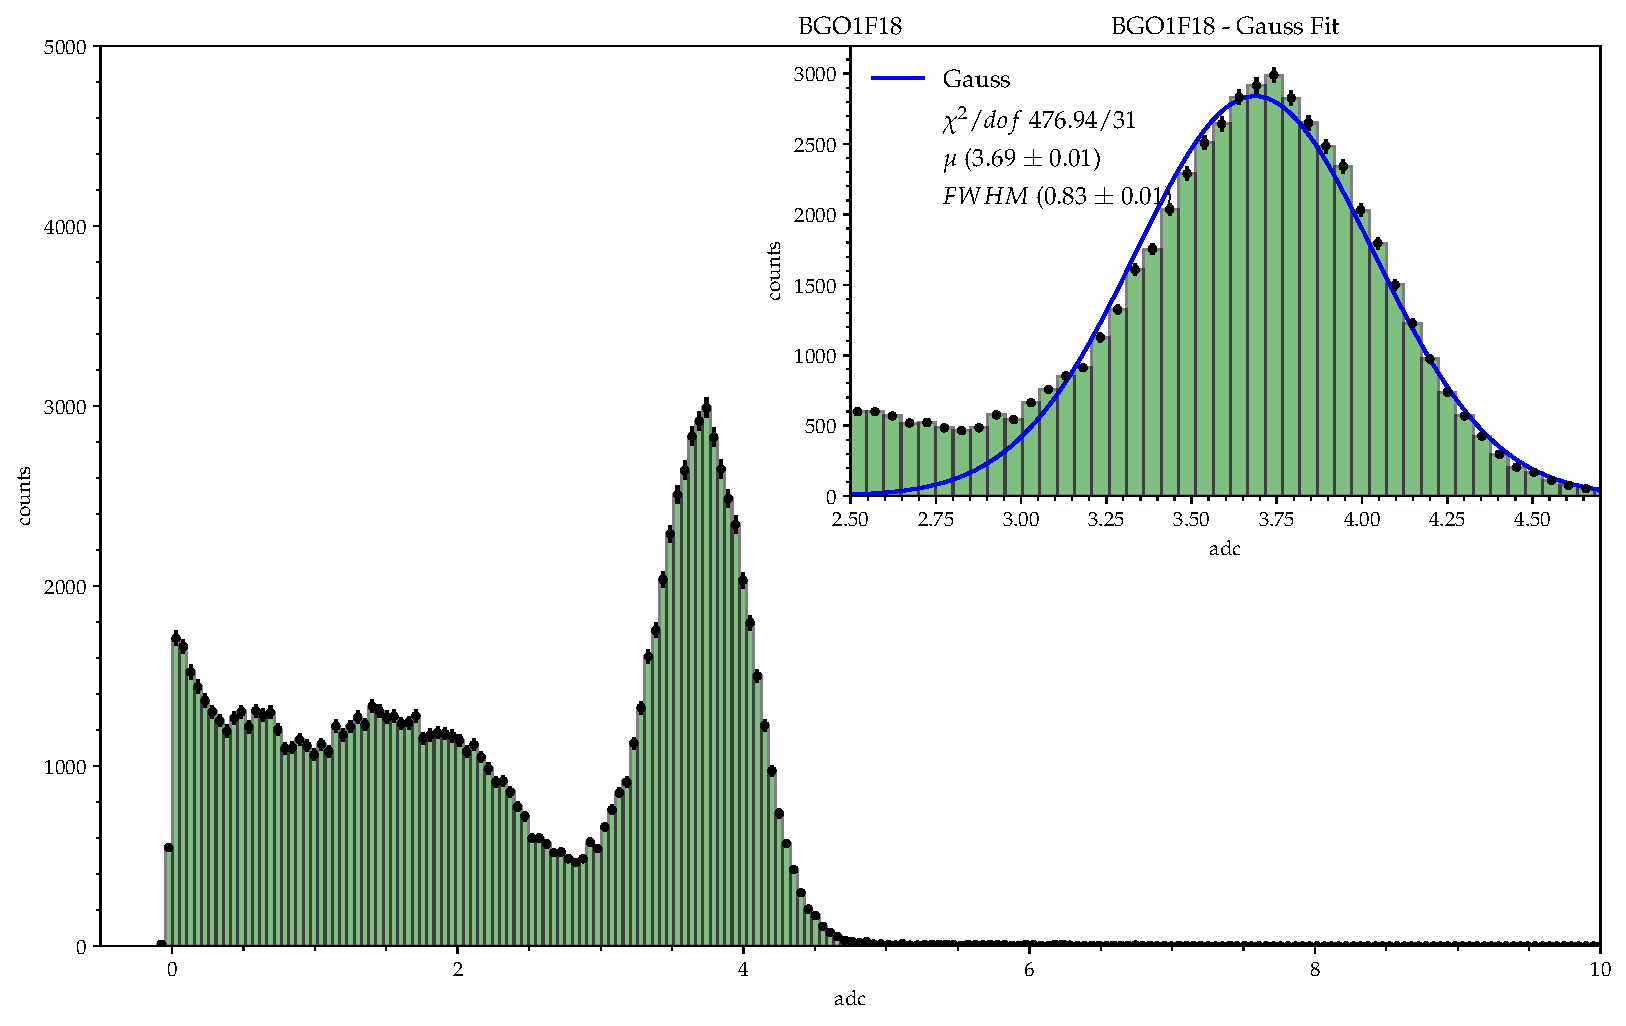
\includegraphics[width=0.80\textwidth]{figure.pdf}
\caption{Figura 1: Rappresentazione schematica della traiettoria percorsa da un neutrone $termico$ durante il suo passaggio all'interno della materia.}
\label{fig:float}
\end{figure*}


%=====================================
% CODICI IN LATEX
%=====================================
\section{Codici in \LaTeX}
Esempio di codice in Python:

\begin{lstlisting}[firstnumber = 54]
		# Importa librerie necessarie
		import random
		import numpy as np
		import math
		
		# Vettore del numero delle collisioni di ciascun neutrone 
		N_coll_vec = np.zeros(N)
	
		# Vettore della distanza TOTALE percorsa dal neutrone prima di essere assorbito da un nucleo 
		d_tot_vec  = np.zeros(N)
	
		# Vettore della distanza tra sorgente - punto finale di arresto
		r_vec      = np.zeros(N)
		
		# Vettore dei tempi di volo 
		t_vec      = np.zeros(N)
\end{lstlisting}

\medskip
Su latex è inoltre possibile caricare direttamente un file contenente del codice (possibilmente \textbf{Python}), che si trovi nella stessa cartella di lavoro e selezionando persino le righe di inizio e di fine che ci interessa importare, come nell'esempio seguente:

\lstset{caption={Titolo 1 al primo file}}
\lstinputlisting[firstline=1,lastline=10]{prova_listing.py}

\lstset{caption={Titolo 2 al secondo file}}
\lstinputlisting[firstline=1,lastline=3]{prova_listing.py}
%=====================================
% TABELLE IN LATEX 
%=====================================
\section{Tabelle in \LaTeX}





%=====================================
% BIBLIOGRAFIA 
%=====================================
\begin{thebibliography}{9}
\bibitem{nome_da_citare} 
Tizio, Caio e Sempronio.
\textit{Opera numero 1}.  
Casa Editrice anno.

\end{thebibliography}
\end{document}